
\documentclass{beamer}

% Configuration of beamer
\usetheme{Copenhagen}
\setbeamertemplate{navigation symbols}{}
\setbeamertemplate{footline}[frame number]

% Basic packages
\usepackage{graphics,graphicx,hyperref,amsmath,amssymb,amsthm,color,multirow}
\usepackage{ragged2e}
\usepackage{verbatim,listings}
\usepackage[normalem]{ulem}
\usepackage{hhline}
\usepackage{xcolor}
%\usepackage{enumitem}
%\newlist{longitem}{itemize}{5}
% \newlist{longenum}{enumerate}{5}
% \setlist[longenum,1]{label=\roman*)}
% \setlist[longenum,2]{label=\alph*)}
% \setlist[longenum,3]{label=\arabic*)}
% \setlist[longenum,4]{label=(\roman*)}
% \setlist[longenum,5]{label=(\alph*)}
\usepackage{colortbl}

\usepackage{textcomp} 
\usepackage[most]{tcolorbox}

\newtcblisting{commandshell}{colback=black,colupper=white,colframe=yellow!75!black,
listing only,listing options={language=sh},
every listing line={\textcolor{green}{\small\ttfamily\bfseries b-an01 [$\sum$/store/bbrydsoe/MPI]\$ }}}


\usepackage{tikz}
\usetikzlibrary{shapes}
\setbeamerfont{block title}{size=\small}
\setbeamerfont{frametitle}{size=\small}

\title[MD simulations with a focus on NAMD - HPC2N intro]{A brief introduction to using Kebnekaise at HPC2N}
% \subtitle{}
%\author{Birgitte Bryds\o, Mirko Myllykoski, Pedro Ojeda-May}
\author{Birgitte Bryds\o}
\institute{HPC2N, Ume\aa{} University}

\titlegraphic{\center{
\includegraphics[height=0.9cm]{figures/umu-logo-left-se.png}\hspace*{0.3cm}~
\includegraphics[height=0.91cm]{figures/SNIC_logo.png}\hspace*{0.3cm}~
\includegraphics[height=0.9cm]{figures/hpc2n.png}\hspace*{0.3cm}~
\includegraphics[height=0.9cm]{figures/prace-logo-icon.png}\hspace*{0.3cm}}
}
\date{\textbf{7}-8 April 2022}
\begin{document}

\frame{
  \titlepage
}

\frame{\frametitle{Overview}

  \begin{block}{}
    \begin{itemize}
%    \item Kebnekaise
    \item Connecting to HPC2N's systems (Kebnekaise) with ThinLinc
    \item Editors
    \item The filesystem 
    \item The module environment
    \item Example: NAMD
    \item Executing a job on Kebnekaise
    \begin{itemize}
      \item SLURM
      \item Jobscript examples
    \end{itemize} 
    \item Important information
    \end{itemize}
  \end{block}
}

% \frame{\frametitle{Kebnekaise}

%   \begin{block}{}
%     \begin{center}
%       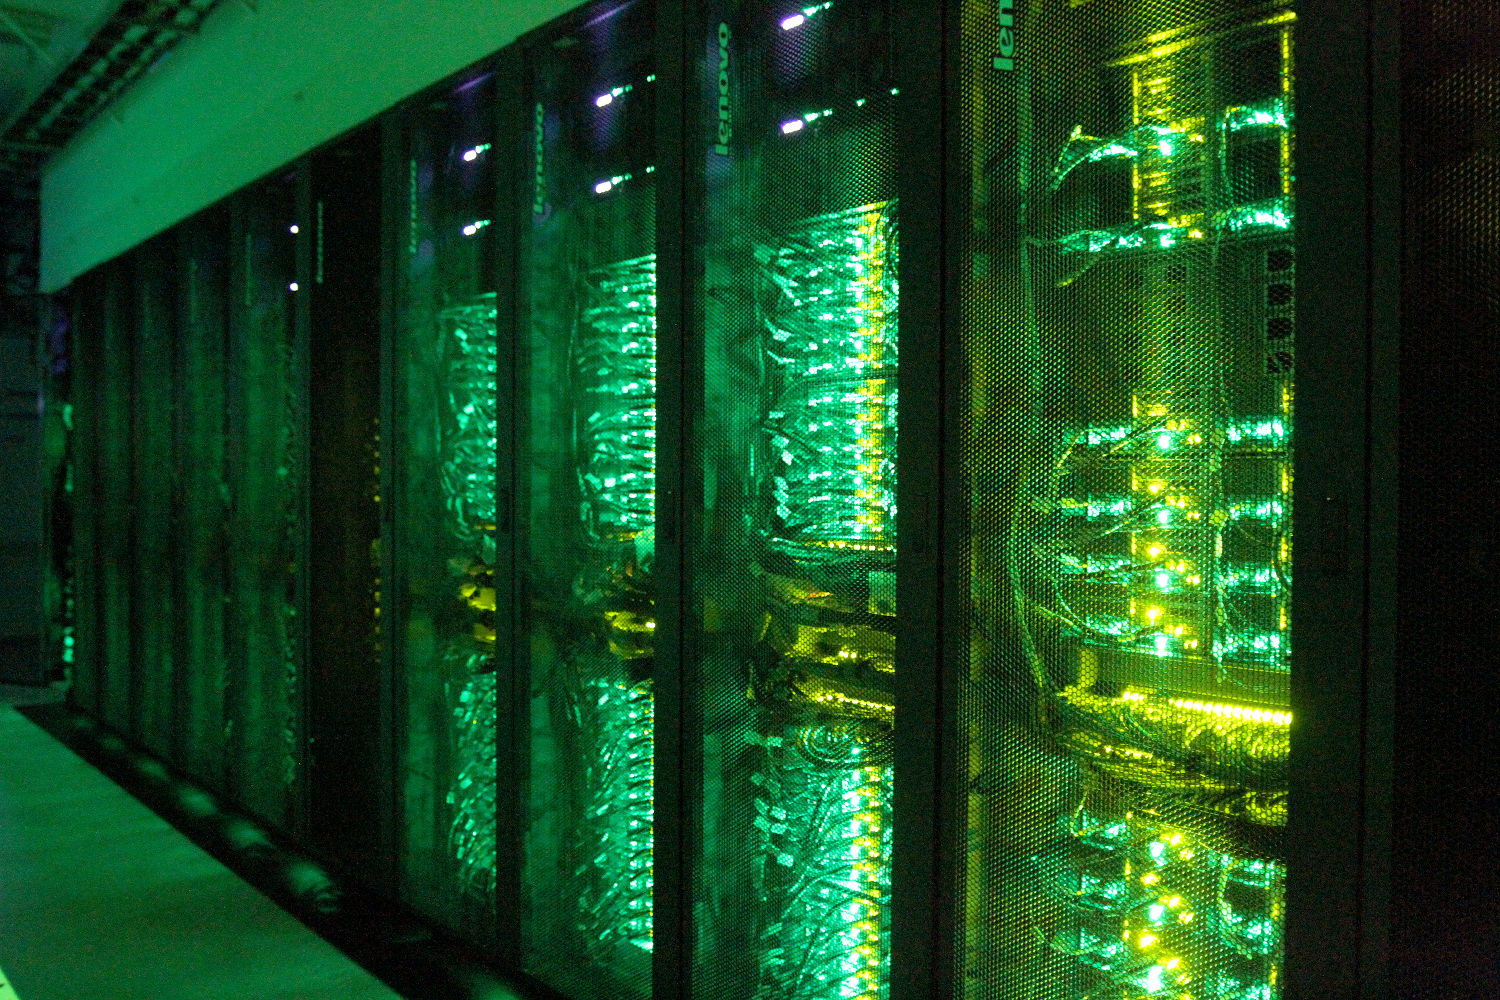
\includegraphics[width=2.4cm]{figures/kebnekaise.png}
%     \end{center}
%   \end{block}

%   \begin{block}{}
%     \begin{enumerate}
%       \begin{footnotesize}
%       \item 602 nodes / 19288 cores (of which 2448 are KNL)
%       \end{footnotesize}
%       \begin{itemize}
%         \begin{scriptsize}
%         \item 432 Intel Xeon E5-2690v4, 2x14 cores, 128 GB/node
%         \item 52 Intel Xeon Gold 6132, 2x14 cores, 192 GB/node
%         \item 20 Intel Xeon E7-8860v4, 4x18 cores, 3072 GB/node
%         \item 32 Intel Xeon E5-2690v4, 2x NVidia K80, 2x14, 2x4992, 128 GB/node
%         \item 4 Intel Xeon E5-2690v4, 4x NVidia K80, 2x14, 4x4992, 128 GB/node
%         \item 10 Intel Xeon Gold 6132, 2x NVidia V100, 2x14, 2x5120, 192 GB/node
%         \item 36 Intel Xeon Phi 7250, 68 cores, 192 GB/node, 16 GB MCDRAM/node
%         \end{scriptsize}
%       \end{itemize}
%       \begin{footnotesize}
%       \item 501760 CUDA ``cores'' (80*4992 cores/K80+20*5120 cores/V100)
%       \item More than 136 TB memory total
%       \item Interconnect: Mellanox FDR / EDR Infiniband
%       \item Theoretical performance/HP Linpack: 984 TF / 791 TF
%       \item Date installed: Fall 2016 / Spring 2017 / Spring 2018 
%       \end{footnotesize}
%     \end{enumerate}
%   \end{block}

% }

\frame{\frametitle{Connecting to HPC2N's systems with ThinLinc}

  \begin{block}{}
    \begin{small}
      ThinLinc is a cross-platform remote desktop server developed by
    Cendio AB. It is especially useful for software with a graphical
    interface.
    \end{small}
  \end{block}{}

  \begin{block}{}
    \begin{itemize}
    \item Download the client and install it: \texttt{https://www.cendio.com/thinlinc/download}. 
    \item Start the client. Enter the name of the server:
      \textbf{kebnekaise-tl.hpc2n.umu.se}. Enter your HPC2N username.
    \item (First time only) Go to "Options" $->$ "Security". Check that authentication is set to password.
    \item (First time only) Go to "Options" $->$ "Screen". Uncheck "Full screen mode".
    \item Enter your HPC2N password. Click "Connect"
    \item Click "Continue" when told that the server's host key is not in the registry. Wait for the ThinLinc desktop to open.
    \end{itemize}
  \end{block}

}

% \frame{\frametitle{Using Kebnekaise}\framesubtitle{Transfer your files and data}

%   \begin{block}{}
%     \begin{itemize}
%     \item \textbf{Linux, OS X:} 
%       \begin{itemize}
%       \item Use scp (or sftp) for file transfer. Example, scp:\\
%         \vspace{2mm}
%         \begin{footnotesize}
%           \texttt{local> scp username@kebnekaise.hpc2n.umu.se:file .}\\
%           \texttt{local> scp file username@kebnekaise.hpc2n.umu.se:file}
%         \end{footnotesize}
%       \end{itemize}
%     \item \textbf{Windows:} 
%       \begin{itemize}
%       \item Download client: WinSCP, FileZilla (sftp), PSCP/PSFTP, ...
%       \item Transfer with sftp or scp
%       \end{itemize}
%     \item \textbf{Mac/OSX:} 
%       \begin{itemize}
%       \item Transfer with sftp or scp (as for Linux) using Terminal
%       \item Or download client: Cyberduck, Fetch, ... 
%       \end{itemize}
%     \item More information in guides (see previous slide) and here: \scriptsize{https://www.hpc2n.umu.se/documentation/filesystems/filetransfer} \normalsize{}
%     \end{itemize}
%   \end{block}

% }


\frame{\frametitle{Editors}

  \begin{block}{}
    \justify
    Editing your files
  \end{block}

  \begin{block}{}
    \begin{itemize}
    \item Various editors: vi, vim, nano, emacs ... 
    \item Example, vi/vim: 
      \begin{itemize}
      \item \texttt{vi $<$filename$>$}
      \item Insert before: i
      \item Save and exit vi/vim: \texttt{Esc :wq} 
      \end{itemize} 
    \item \textbf{Example, nano:} 
      \begin{itemize}
      \item \texttt{nano $<$filename$>$}
      \item Save and exit nano: \texttt{Ctrl-x} 
      \end{itemize} 
    \item Example, Emacs: 
      \begin{itemize}
      \item Start with: emacs 
      \item Open (or create) file: \texttt{Ctrl-x Ctrl-f}
      \item Save: \texttt{Ctrl-x Ctrl-s}
      \item Exit Emacs: \texttt{Ctrl-x Ctrl-c}
      \end{itemize} 
    \end{itemize}
  \end{block}
}

\frame{\frametitle{The filesystem}

   \begin{block}{}
     \justify
     More info here: http://www.hpc2n.umu.se/filesystems/overview
   \end{block}

 \begin{block}{}
  \begin{scriptsize}
    \begin{tabular}{|c|>{\columncolor[RGB]{255, 255, 102}}c|c|c|}
    \hline
   & & & \\ 
      & \textbf{Project storage} & \textbf{\$HOME (25GB)} & \textbf{/scratch} \\
     & & & \\ \hhline{|=|=|=|=|} 
   Recommended & & & \\
   for batch jobs & Yes & (No, size) & Yes \\ \hline 
   Backed up & No & Yes & No \\ \hline 
   Accessible & & & \\
   by batch & Yes & Yes & Yes (node only) \\ 
   system & & & \\ \hline 
   Performance & High & High & Medium \\ \hline 
   Default & & & \\
   readability & Group only & Owner & Owner \\ \hline 
   Permissions & & & \\ 
   management & chmod, chgrp, ACL & chmod, chgrp, ACL & N/A for batch jobs \\ \hline 
     & Storage your group & & \\
     Notes & get allocated through & Your home- & Per node \\
     & the storage projects & directory & \\
   \hline
  \end{tabular}
 \end{scriptsize}
   \end{block} 
   
 }

 \frame{\frametitle{The filesystem, example}

   \begin{block}{}
     \justify
     The course project has default storage here: \\
     /proj/nobackup/snic2022-22-237 
   \end{block}

 \begin{block}{}
You should create a sub-directory under this directory, for your
storing own files for this course, and for running the exercises: \\
\begin{itemize}
  \item \texttt{cd /proj/nobackup/snic2022-22-237}
  \item \texttt{mkdir $<$username$>$}  (or whatever you want to call your
  directory)
\end{itemize}

This storage will only be available for a few weeks (until around 1
May 2022).  
   \end{block} 
   
   }
   
\frame{\frametitle{The Module Environment} 

  \begin{block}{}
    \justify
    \begin{footnotesize}
      Most programs are accessed by first loading them as a 'module'
      \end{footnotesize}
  \end{block}

  \begin{block}{}
    \begin{footnotesize}
    Modules are:
    \begin{itemize}
    \item used to set up your environment (paths to executables, libraries, etc.) for a particular (set of) software package(s)
    \item for helping users manage their Unix/Linux shell environment, allowing groups of related environment-variable settings to be made or removed dynamically 
    \item allows having multiple versions of a program or package available by just loading the proper module 
    \item installed in a hierarchial layout; thus some modules are
      only available after loading a specific compiler and/or MPI version
    \end{itemize}
\textbf{Compiler toolchains} load software-bundles for a complete
environment (compiling, using prebuilt software). Includes some/all of: compiler
        suite, MPI, BLAS, LAPACK, ScaLapack, FFTW, CUDA.
        \begin{itemize}
        \item \textbf{foss}: GCC, OpenMPI, OpenBLAS/LAPACK, FFTW, ScaLAPACK
        \item \textbf{intel}:  icc, ifort, IntelMPI, IntelMKL
        \end{itemize}
      \end{footnotesize}
  \end{block}
}


% \frame{\frametitle{Compiling and running MPI on Kebnekaise at
%     HPC2N}\framesubtitle{The Module Environment} 

%   \begin{block}{}
%     \justify
% Quick overview - for reference
%   \end{block}

%   \begin{block}{}
%     \begin{itemize}
%       \begin{footnotesize}
%       \item See which modules exists: \\ 
%         \texttt{module spider} or \texttt{ml spider} 
%       \item Modules depending only on what is currently loaded: \\ 
%         \texttt{module avail} or \texttt{ml av}
%       \item See which modules are currently loaded: \\ 
%         \texttt{module list} or \texttt{ml} 
%       \item Example: loading a compiler toolchain and version, here for GCC, OpenMPI, OpenBLAS/LAPACK, FFTW, ScaLAPACK and CUDA: \\ 
%         \texttt{module load fosscuda/2021a} or \texttt{ml fosscuda/2021a} 
%       \item Example: Unload the above module:\\ 
%         \texttt{module unload fosscuda/2021a} or \texttt{ml -fosscuda/2021a}
%       \item More information about a module: \\ 
%         \texttt{module show $<$module$>$} or \texttt{ml show $<$module$>$} 
%       \item Unload all modules except the 'sticky' modules: \\ 
%         \texttt{module purge} or \texttt{ml purge}
%       \end{footnotesize}
%     \end{itemize}
%   \end{block}
% }


% \frame{\frametitle{Compiling and running MPI on Kebnekaise at
%     HPC2N}\framesubtitle{The Module Environment} 

%   \begin{block}{}
%     \justify
%     \begin{small}
%       \textbf{Compiler toolchains} load bundles of software making up a complete environment for compiling/using a specific prebuilt software. Includes some/all of: compiler suite, MPI, BLAS, LAPACK, ScaLapack, FFTW, CUDA. 
%     \end{small}
%   \end{block}

%   \begin{block}{}
%     \begin{itemize}
%       \begin{footnotesize}
%       \item Toolchains for Intel and GCC are available at
%         HPC2N. Below are some of the more common ones. Check
%         \texttt{ml av} for all toolchains, and \texttt{ml spider
%           $<$toolchain$>$} for available versions:
%       \end{footnotesize}
%       \begin{itemize}
%         \begin{footnotesize}
%         \item \textbf{foss}: GCC, OpenMPI, OpenBLAS/LAPACK, FFTW, ScaLAPACK
%         \item \textbf{fosscuda}: GCC, OpenMPI, OpenBLAS/LAPACK, FFTW, ScaLAPACK, and CUDA
%         \item \textbf{gomkl}: GCC, OpenMPI, IntelMKL
%         \item \textbf{gompi}: GCC, OpenMPI
%         \item \textbf{gompic}: GCC, OpenMPI, CUDA
%        \item \textbf{iimpi}: icc, ifort, IntelMPI
%         \item \textbf{intel}: icc, ifort, IntelMPI, IntelMKL
%         \item \textbf{intelcuda}: intel and CUDA
%           \item \textbf{iompi}: icc, ifort, OpenMPI
%          \end{footnotesize}
%       \end{itemize}
%     \end{itemize}
%   \end{block}
% }



\frame{\frametitle{Finding software modules to load} 

  \begin{block}{}
    \begin{itemize}
    \item Listing all available modules: \\ \texttt{module spider / ml spider}
    \item Listing all versions of a software: \\ \texttt{module
      spider $<$software$>$ / ml spider $<$software$>$}
      \begin{itemize}
      \item Example: NAMD \\
      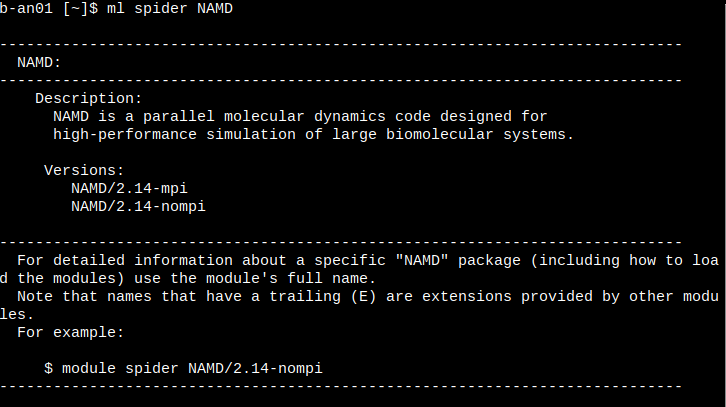
\includegraphics[width=7cm]{figures/load-namd.png}
    \end{itemize}
    \end{itemize}
\end{block}

}



\frame{\frametitle{Loading and unloading software modules} 

  \begin{block}{}
    \begin{footnotesize}
      \begin{itemize}
    \item Loading a module: \\
      \begin{itemize}
    \begin{footnotesize}
        \item Most software modules have prerequisites. Use 'ml
          spider' on a specific version to see how it is loaded
        \item \texttt{ml spider $<$software$>$/version}
          \item Then load it and any prerequisites
      \texttt{module load $<$pre-requisite module$>$ / ml $<$pre-requisite module$>$}
      \texttt{module load $<$module$>$ / ml $<$module$>$}
      \item You can also load all on one line, listing the
        prerequisites first (\texttt{ml $<$pre-requisite module$>$ $<$module$>$})
    \end{footnotesize}
     \end{itemize}
    \item Unloading a module: \\
      \texttt{module unload $<$module$>$}
    \item Unloading all modules: \\
      \texttt{module purge / ml purge}
    \item Seeing which modules you currently have loaded \\
      \texttt{module list / ml}
    \end{itemize}
    \end{footnotesize}
\end{block}

}

\frame{\frametitle{Loading software modules: example}

  \begin{block}{}
    Loading NAMD/2.14-mpi:
    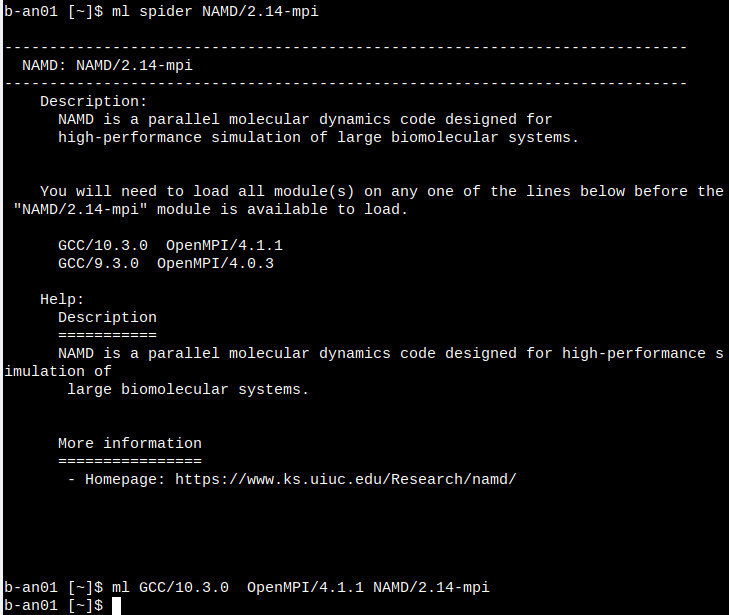
\includegraphics[width=8cm]{figures/load-namd-version.png}
    \end{block}

}

\frame{\frametitle{Loaded software modules: example, NAMD/2.14-mpi}

  \begin{block}{}
    Checking which modules we have loaded now: 
    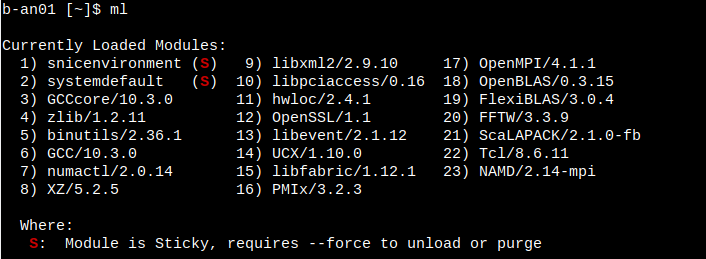
\includegraphics[width=7cm]{figures/namd-loaded.png}
    \end{block}

}

% \frame{\frametitle{Compiling and running MPI on Kebnekaise at
%     HPC2N}\framesubtitle{Examples, GNU} 

%   \begin{block}{}
%     \begin{itemize}
%     \item MPI C program
%       \begin{itemize}
%       \item \texttt{mpicc -O3 -march=native -o program program.c}
%       \end{itemize}
%     \item MPI F90 program
%       \begin{itemize}
%       \item \texttt{mpif90 -O3 -march=native -o program program.f90}
%       \end{itemize}
%     \item The options in both cases mean:
%       \begin{enumerate}
%       \item \texttt{-03} optimization level 3
%       \item \texttt{-march=native} optimized for our CPUs
%       \item \texttt{-o program} names the ouput '\texttt{program}'
%       \end{enumerate}
%     \item You can use the options for the underlying compiler       
%     %  \item mpirun -np N hello
%     %     \item where N $<=$ number of MPI tasks you asked for in your job
%     %     \end{itemize}
%     %   \item MPI F90 program
%     %     \begin{itemize}
%     %     \item
%     %     \end{itemize}
%     %   \end{itemize}
%     % \end{itemize}
%     \end{itemize}
%   \end{block}
% }

% \frame{\frametitle{Compiling and running MPI on Kebnekaise at
%     HPC2N}\framesubtitle{Examples, Intel} 

%   \begin{block}{}
%     \begin{itemize}
%        \item MPI C program
%           \begin{itemize}
%           \item \texttt{mpiicc -O3 -xHost -o program program.c}
%           \end{itemize}
%        \item MPI F90 program
%          \begin{itemize}
%          \item \texttt{mpiifort -O3 -xHost -o program program.f90}
%          \end{itemize}
%          \item The options in both cases mean: 
%            \begin{enumerate}
%            \item \texttt{-03} optimization level 3 
%            \item \texttt{-xHost} builds for our CPUs
%            \item \texttt{-o program} names the output '\texttt{program}'
%            \end{enumerate}
%            \item You can use the options for the underlying compiler 
%       \end{itemize}
%  \end{block}
% }

% \frame{\frametitle{Compiling and running MPI on Kebnekaise at
%     HPC2N}\framesubtitle{Running MPI programs} 

%   \begin{block}{}
%     \begin{itemize}
%     \item Ensure the compiler and MPI modules are loaded (\texttt{foss/2021a}
%       or \texttt{intel/2021a}) 
%     \item MPI jobs must be run through the batch system (SLURM)
%       \begin{itemize}
%       \item This will be the case for most (all?) HPC systems
%         \end{itemize}
%     \item When submitting jobs to the batch system, you \textbf{must}
%       use the course project! 
%     \item To run the MPI program, you use \texttt{srun -n ./program}
%       inside the batch script. 
%       \begin{itemize}
%          \item \texttt{-n} is the number of MPI tasks. It can be 1 to
%            number of tasks you asked for when submitting the job. If
%            omitted, you will use the number of tasks asked for in the
%            job. 
%          \end{itemize}
%        \end{itemize}
%   \end{block}
% }

\frame{\frametitle{The Batch System (SLURM)}

  \begin{block}{}
    \begin{itemize}
    \item Large/long/parallel jobs must be run through the batch system 
    \item SLURM is an Open Source job scheduler, which provides three key functions
      \begin{itemize}
      \item Keeps track of available system resources
      \item Enforces local system resource usage and job scheduling policies
      \item Manages a job queue, distributing work across resources according to policies
      \end{itemize}
    \item In order to run a batch job, you need to create and submit a SLURM submit file (also called a batch submit file, a batch script, or a job script). 
    \item Guides and documentation at: http://www.hpc2n.umu.se/support
    \end{itemize}
  \end{block}
}


 \frame{\frametitle{Useful commands to the Batch System (SLURM)}

   \begin{block}{}
     \begin{itemize}
     \item Submit job: \texttt{sbatch $<$jobscript.sh$>$} (successful
       submission returns a job-id number) \\
       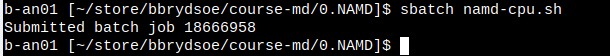
\includegraphics[width=5cm]{figures/submit.png}
       \item As default, output/errors are found in \texttt{slurm-$<$job-id$>$.out} 
     \item Get list of all jobs: \texttt{squeue}
     \item Get list of only your jobs: \texttt{squeue -u $<$username$>$} \\
       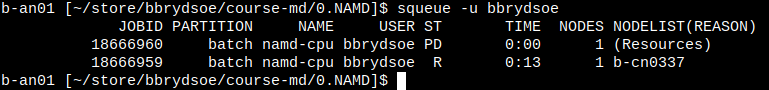
\includegraphics[width=6cm]{figures/squeue.png}
     \item Adding the flag \texttt{--start} to \texttt{squeue} gives
         the estimated job start time. This can change depending on
         other people's jobs. 
     \item Check on a specific job: \texttt{scontrol show job $<$job id$>$} 
     \item Delete a specific job: \texttt{scancel $<$job id$>$}
       \item Delete all your jobs: \texttt{scancel -u $<$username$>$}
 %    \item Useful info about job: \texttt{sacct -l -j  $<$jobid$>$ $|$ less -S}
     \end{itemize}
   \end{block}
 }

 \frame{\frametitle{SLURM batch script for a standard NAMD job (CPU)} 

    \begin{block}{}
      \begin{small}
        \texttt{\#!/bin/bash} \\
        \texttt{\#SBATCH -A SNIC2022-22-237} \texttt{\textcolor{red}{\#Project id}} \\
        \texttt{\#SBATCH -J my-namd-job} \texttt{\textcolor{red}{\#Name of job}} \\
          \texttt{\#SBATCH --time=00:10:00} \texttt{\textcolor{red}{\#Jobtime (HH:MM:SS) Max: 168H}}\\
          \texttt{\#SBATCH -N 1} \texttt{\textcolor{red}{\#Number of nodes. }} \\
          \texttt{\#SBATCH -n 28} \texttt{\textcolor{red}{\#Number of processes. }} \\
 %         \hspace{2.5cm}  Default is 1 CPU/task. \texttt{\textcolor{red}{Change with --cpus-per-task}} \\
        \vspace{3mm} 
        \texttt{ml purge $<$ /dev/null 2$>$\&1} \\ 
        \texttt{ml GCC/10.3.0  OpenMPI/4.1.1} \\
        \texttt{ml NAMD/2.14-mpi} \\
        \vspace{3mm}
        \texttt{mpirun -np 28 namd2 config-file.inp > output\_cpu.dat}
      \end{small}
    \end{block}

    \begin{block}{}
      \textbf{NOTE} if you are using the reservation for this course, you
      \textbf{have} to add \texttt{\#SBATCH --gres=gpu:k80:2} (since the
      reservation is only for GPU nodes)
    \end{block}
    
 }

 \frame{\frametitle{SLURM batch script for a standard NAMD job (GPU)} 

    \begin{block}{}
      \begin{small}
        \texttt{\#!/bin/bash} \\
        \texttt{\textcolor{red}{\#Project id}} \\
        \texttt{\#SBATCH -A SNIC2022-22-237}
        \texttt{\#SBATCH -J my-namd-job} \texttt{\textcolor{red}{\#Name of job}} \\
          \texttt{\#SBATCH --time=00:10:00}
          \texttt{\textcolor{red}{\#Jobtime (HH:MM:SS) Max: 168H}}\\
          \texttt{\#SBATCH -N 1} \texttt{\textcolor{red}{\#Number of nodes. }} \\
          \texttt{\#SBATCH -n 28} \texttt{\textcolor{red}{\#Number of processes. }} \\
          \texttt{\#SBATCH --gres=gpu:k80:2} \texttt{\textcolor{red}{\#Asking for 2 K80 GPUs}} \\
          \texttt{\#SBATCH --exclusive} \texttt{\textcolor{red}{\#Asking for exclusive access to the node}}\\
        \vspace{3mm} 
        \texttt{ml purge $<$ /dev/null 2$>$\&1} \\ 
        \texttt{ml GCC/9.3.0  CUDA/11.0.2  OpenMPI/4.0.3} \\
        \texttt{ml NAMD/2.14-nompi} \\
        \vspace{3mm}
        \texttt{namd2 +p28 config-file.inp > output\_gpu.dat}
      \end{small}
    \end{block}

 }


 \frame{\frametitle{Various useful info}

   \begin{block}{}
     \begin{small}
       \begin{itemize}
     \item A project has been set up for the workshop: \texttt{SNIC2022-22-237}
     \item Use it by adding this to your submit file: \\
       \texttt{\#SBATCH -A SNIC2022-22-237} \\
       \item The project is ONLY valid during the course and a
         few weeks after. 
       \item Default storage is included with the project. It can be found
         here: \texttt{/proj/nobackup/snic2022-22-237} 
       \item There is a reservation. To use, add this to the submit file: \\ 
       \textbf{THURSDAY} \\
       \texttt{\#SBATCH --reservation=namd-gpu-day1} \\
       \textbf{FRIDAY} \\
       \texttt{\#SBATCH --reservation=namd-gpu-day2} 
     \item The reservation is ONLY valid for the specific day of the course.
     \end{itemize}
     \end{small}
   \end{block}

 }

\end{document}






